\documentclass[12pt, letterpaper]{article}
\usepackage{fancyhdr}
\usepackage{graphicx} % Required for inserting images
\graphicspath{{images/}} 
\usepackage{color}
\usepackage[sort&compress]{natbib}
\usepackage[colorlinks, urlcolor= blue]{hyperref}
\title{{\color{blue}JPEG IMAGE COMPRESSION STANDARD}}
\author{\textbf{Under the  guidance of Sir Manish K Gupta}\\\\Aditya Raina - 202201466\\Om Lachake - 202201017\\Parjanya Rajput -202201115\\Ayushi Jani - 202201141\\Harshali Dharmik - 202201214\\Pari Chauhan - 202201189}
\date{May 2023}

\begin{document}

\pagestyle{fancy}

\maketitle

\begin{center}
    
\includegraphics{DAIICT-Logo} 
\end{center}
\newpage
\fancyfoot[C]{\thepage}
\tableofcontents{}
\newpage
\begin{abstract}
    This project report provides a comprehensive exploration of JPEG compression, a widely used technique for efficiently storing and transmitting digital images. It discusses the core principles behind JPEG, including lossy compression, chroma subsampling, the Discrete Cosine Transform (DCT), quantization, and Huffman coding. The report highlights the trade-off between file size reduction and image quality and emphasizes that JPEG is most effective for natural images. By understanding the intricacies of JPEG compression, users can make informed decisions to achieve an optimal balance between file size and image fidelity. Overall, the project aimed to deepen understanding of JPEG compression techniques for practical applications.
\end{abstract}

\section{{\color{blue}Introduction}}
\paragraph{}\textit{In today's computer-centric world, the significance of storage as a crucial aspect cannot be overlooked. With the exponential growth of digital data, the need for efficient data compression techniques has become increasingly paramount.} 
\paragraph{}\textit{Programs using complex graphics are showing up in virtually every area of computing applications including games, education, desktop publishing, graphical design, and most recently the World Wide Web. Although graphics do a great deal to enhance the usability and visual aesthetics of such applications, they consume prodigious amounts of disk storage.}
\paragraph{}\textit{Data compression plays a pivotal role in optimizing storage utilization by reducing the size of files and data streams. By employing various algorithms and methodologies, compression algorithms aim to eliminate redundant or irrelevant information, enabling more efficient data representation and transmission.}

\paragraph{}\textit{Efficient data compression not only conserves storage space but also enhances data transfer speeds, as smaller file sizes facilitate faster transmission and retrieval. Furthermore, compressed data requires less bandwidth, making it advantageous for applications that involve limited network resources or bandwidth-constrained environments.}

\paragraph{}\textit{In conclusion data storage efficiency can’t be overlooked as it helps in enhancing data transmission, optimized storage capacity and overall system performance. Let’s dive into the inner workings of many components involved.}

\section{{\color{blue}Image Compression}}
\textit{Image compression is a method of data compression on digital images. The main objective in image compression : }
\begin{itemize}
    \item \textit{ Efficient data storage }
    \item \textit{  Transmission of data in efficient form.}
\end{itemize}
\textit{There are two main types of image compression :}
\begin{itemize}
    \item \textit{Lossless }
    \item \textit{Lossy}
\end{itemize}
\subsection{{\color{gray}Lossless}}
\textit{In lossless compression all the information is preserved but the compression rate is low. Lossless compression may range from about 66\% to 33\%. Examples of lossless compressions are Portable network graphic (PNG) and Picture Exchange (PCX). }
\subsection{{\color{gray}Lossy}}
\textit{ To get higher compression rate we use lossy compression, one setback of this type of compression is we are going to deliberately lose information. The compression rate is up to 5\%. Example of this type of compression is JPEG (Joint Photographic Experts Groups). }
\paragraph{}\textit{By the late 1980s, extensive research pushed the development of lossy compression algorithms that take advantage of known limitations of the human eye. Such algorithms play on the idea that slight modifications and loss of information during the compression/decompression process often do not affect the quality of the image as perceived by the human user. \\The JPEG specification includes separate lossy and lossless algorithms; however, the lossless algorithm is rarely used due to its poor compression ratios. Thus, when one mentions JPEG compression, it can almost be assumed that the reference is being made to the lossy algorithm, or the JPEG baseline algorithm. The baseline algorithm, which is capable of compressing continuous tone images to less that 10\% of their original size without visible degradation of the image quality, is detailed below.}

\section{{\color{blue}Images}}
\textit{Let's talk about how computers represent images. Digital images typically use a representation called RGB, which stands for red, green, and blue. Each pixel in an image stores color information using these three-color channels. The intensity of each channel is typically represented by an 8-bit value, ranging from 0 to 255. Higher values indicate a greater intensity or weight of that color channel. }
\begin{center}
    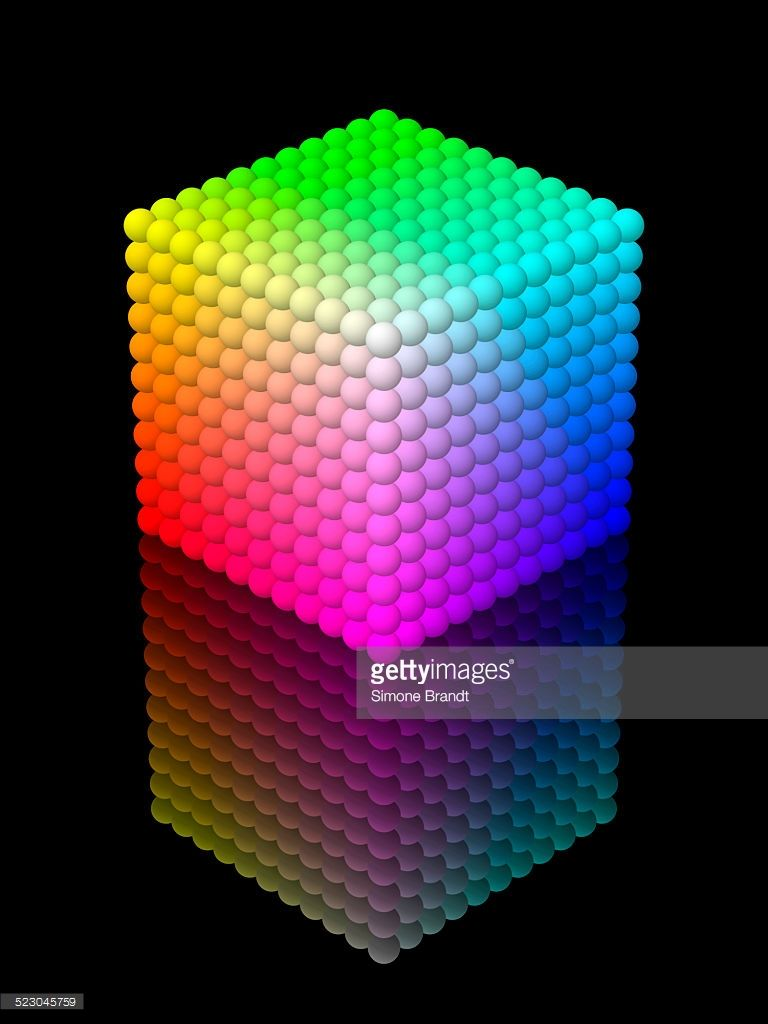
\includegraphics{Image 1(2)} 
\end{center}

\paragraph{}\textit{The combination of the intensity values for the red, green, and blue channels determines the overall color of a pixel. For instance, an RGB value of (255, 0, 0) represents pure red, (0, 255, 0) represents pure green, and (0, 0, 255) represents pure blue. }
\paragraph{}\textit{By adjusting the intensity values of the RGB channels for each pixel, a wide variety of colors and shades can be achieved. The collective arrangement of these RGB values across all pixels forms the complete image displayed on a digital screen.\\If each color occupies 8 bits or a single byte of memory, an image would have 3 bytes per pixel. }
\begin{center}
    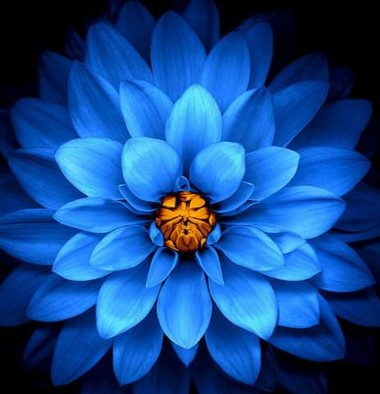
\includegraphics{Flower.2} 
\end{center}
\paragraph{}Here’s an image of 360000 pixels. Based on above information, the size of the image would be 1.08MB. But utilizing JPEG compression reduces its size to 32KB. Same number of pixels but 3\% of expected size. (Note : The image is not upto scale)
\paragraph{}\textit{Since we are dealing with lossy compression, we will lose information. So, the question arises,}\textbf{What sort of information are we going to get rid of? }
\paragraph{}\textit{Scientists have discovered that our eyes are more sensitive to brightness than to color, our eyes are less sensitive to high frequencies.JPEG takes advantages of these points to carry the compression procedure. Let’s dive into these procedures.}
\paragraph{}\textit{JPEG uses technique based on RGB color space known as YCbCr color space. It represents color as combination of three combinations. Y (Luma or brightness),Cb(Chroma Blue), Cr(Chroma Red) }
\paragraph{}\textit{Y (Luma) represents the image’s brightness or grayscale information. It is obtained from the original RGB color space combining red, green and blue channels weighted averages that approximate human perception of brightness. The Y component is usually represented as grayscale image. }
\paragraph{}\textit{Chroma Blue (Cb): The Cb (color blueness) component represents the difference between the blue color component (B) and the luma (Y) component. It provides information about the color blue relative to the brightness of the image.  }
\paragraph{}\textit{Chroma Red (Cr): The Cr (color redness) component represents the difference between the red color component (R) and the luma (Y) component. It provides information about the color red relative to the brightness of the image.}
\paragraph{}\textit{It can be said that Chroma components are going to encode the colors.}
\paragraph{}The provided link can be used to see the effects of Y,Cb and Cr.\url{ goo.gle/yuv}.
\paragraph{}\textit{The human eyes are more sensitive to changes in brightness more than changes in color, so JPEG takes advantage of this by allocating more bits for the luminance component (Y) and fewer bits for the chroma components (Cb and Cr). Thus, the chrominance components are down-sampled to save some space. This technique is known as chroma subsampling or down- sampling. }
\paragraph{}\textit{Another characteristic of human visual system is the frequency contrast sensitivity, that our eyes are more sensitive to changes in high-frequency than changes in low frequency. We are more frequent to miss smaller objects and details as compare to larger objects and details. In other words, low contrast and high frequency parts are barely visible to us. This phenomenon thus allows us to do the compression in the less visible areas. }
\section{{\color{blue}Algorithm}}
\paragraph{}\textit{The JPEG lossy compression algorithm consists of three successive stages, shown in the flow chart below.}

\paragraph{}\textit{DCT Transformation \rightarrow Coeff Quantization \rightarrow Lossless Compression}

\paragraph{}\textit{Both DCT transformation and the final compression of the quantized data are, for the most part, lossless procedures (negligible precision may be lost during DCT transformation due to minor numerical round-offs). This leaves the coefficient quantization phase as the driving force behind JPEG’s overall "lossyness". It is in this step that insignificant data concerning the image is discarded. All three stages are described next.}
\subsection{ChromaDownsampling}
\paragraph{}\textit{Our eyes being less sensitive to color we can sample out Cb and Cr components from an image to reduce the size, this sampling of Cb and Cr components from and image is termed as “Chroma Downsampling/Subsampling”.}
\paragraph{}\textit{We simply go through the image in 2x2 blocks. Each block has 4 pixels with different color values. Now take the average of all 4 pixels and make it the color of one 2x2 block. So, we reduced 4 pixels to 1 pixel just by averaging the values. One may take the values as the value of whole pixel. This way averaging plays a key role in compression. This is only done for Chroma Components}
\subsection{DCT(Discrete Cosine Transform)}
\paragraph{}\textit{A discrete cosine transform (DCT) represents a finite sequence of data points in terms of a sum of cosine functions at different frequencies. It is widely used in signal processing and data compression such as JPEG, MPEG, MP3 etc.}
\paragraph{}\textit{According to the DCT, if we consider an image signal consisting of 8 pixels in length, we can effectively represent it using 8 cosine waves, each having a distinct frequency. This representation allows us to capture the essential information contained within the image while minimizing the amount of data required for storage or transmission. }
\paragraph{}\textit{The DCT achieves this by converting the spatial information of the image into frequency-domain information. It calculates the cosine coefficients for each frequency component and expresses the image as a linear combination of these cosine waves. The resulting DCT coefficients represent the image's energy distribution across different frequency bands.}
\paragraph{}\textit{The 8 different cosine waves are as follows: }
\begin{figure}
\begin{subfigure}
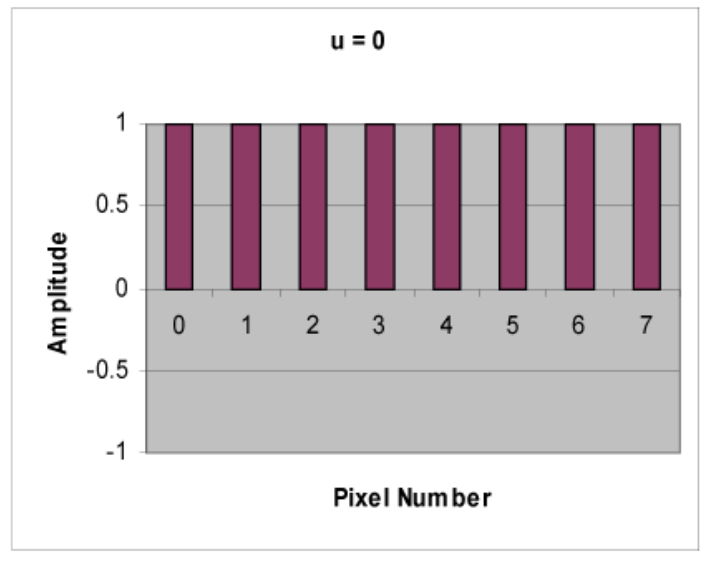
\includegraphics[width=0.5\linewidth, height=6cm]{images/c0.0.png} 
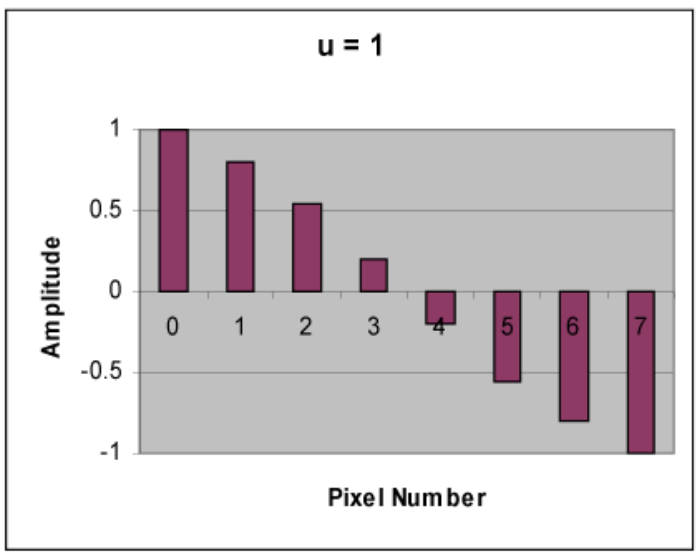
\includegraphics[width=0.5\linewidth, height=6cm]{images/c0.1.png}
\end{subfigure}
\begin{subfigure}
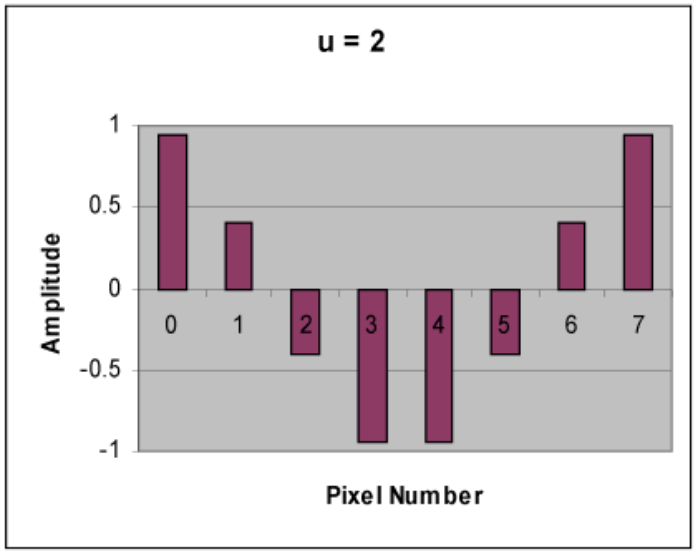
\includegraphics[width=0.5\linewidth, height=6cm]{images/c0.2.png}
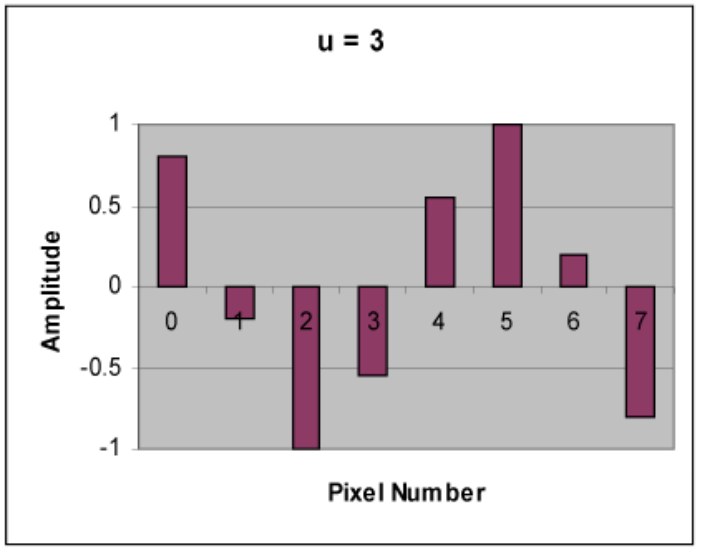
\includegraphics[width=0.5\linewidth, height=6cm]{images/c0.3.png}
\end{subfigure}
\caption{source- cs.standford.edu}
\end{figure}
\begin{figure}
\begin{subfigure}
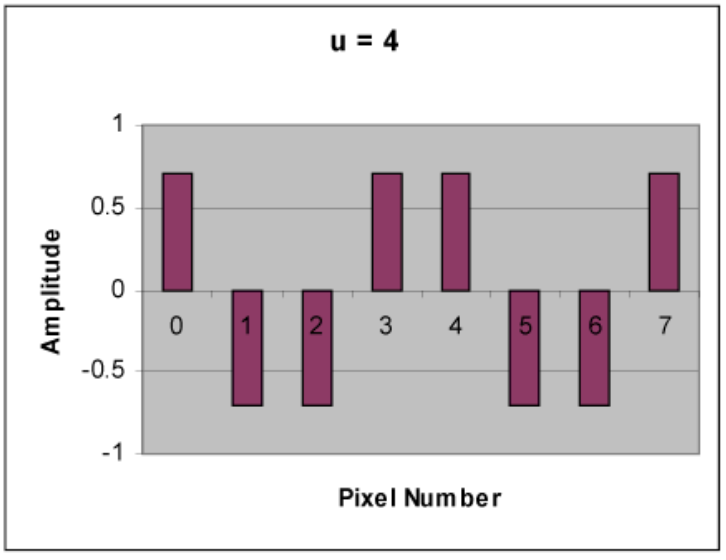
\includegraphics[width=0.5\linewidth, height=6cm]{images/c0.4.png}
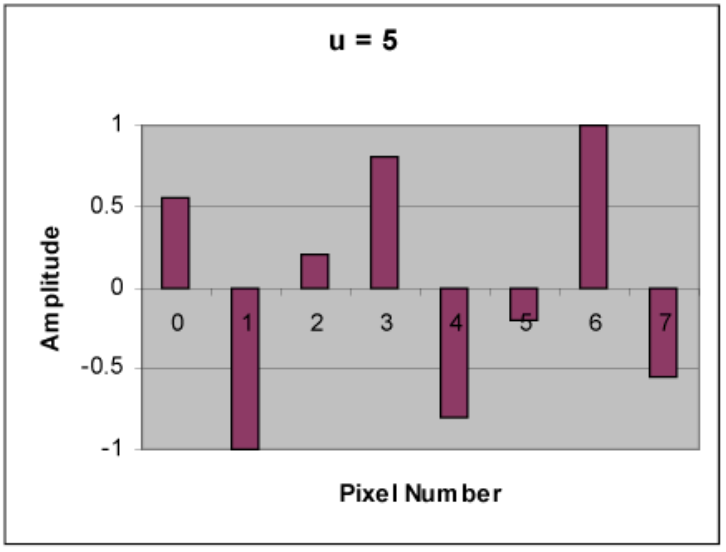
\includegraphics[width=0.5\linewidth, height=6cm]{images/c0.5.png}
\end{subfigure}
\begin{subfigure}
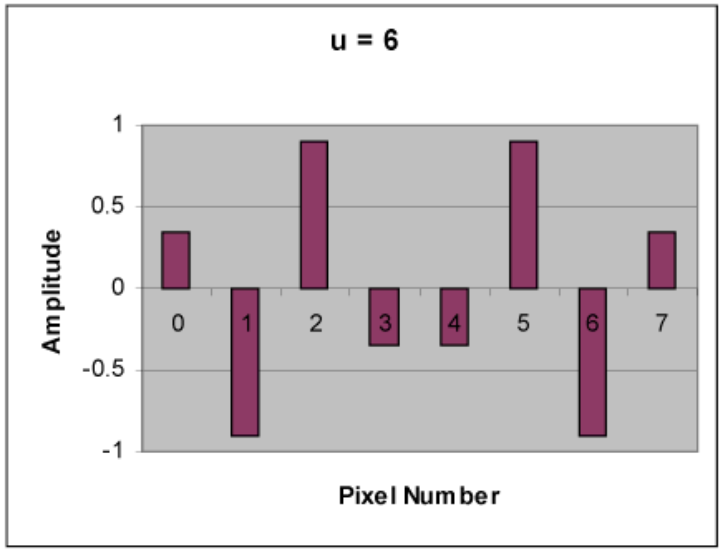
\includegraphics[width=0.5\linewidth, height=6cm]{images/c0.6.png}
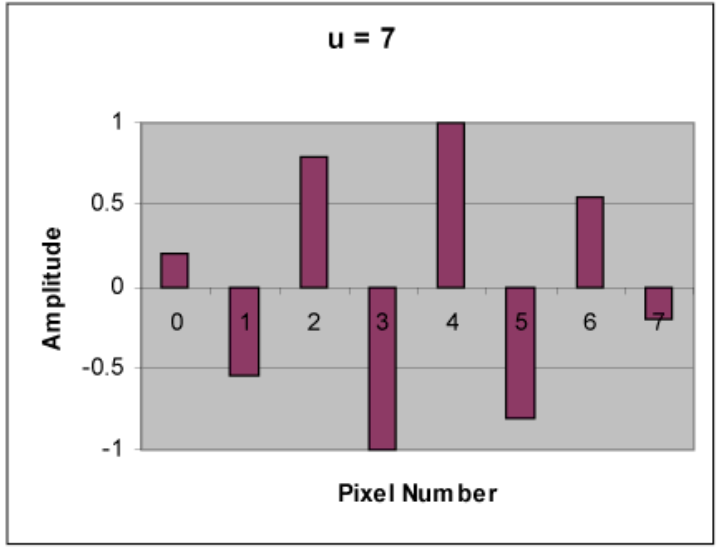
\includegraphics[width=0.5\linewidth, height=6cm]{images/c0.7.png}
\end{subfigure}
\caption{source- cs.standford.edu}
\end{figure}

\paragraph{}\textit{\\In JPEG compression, the image is broken into 8 x 8 groups, each containing 64 pixels. The range of a single byte is between 0 (darkest) and 255 (brightest).  Thus, by removing the high frequency components the size can be reduced. DCT does this by comparing each one of the 8x8 unit with a 64 frequency patterns (where the spatial frequency increases from top-to-bottom and left-to-right).  This process decomposes the image into its frequency components, converting an 8x8 unit where each element represents a brightness level into another 8x8 unit where each element represents the presence of a particular frequency component.}
\paragraph{}\textit{Each of those pixel groups (initial image which was divided into 8 X 8) is separately encoded with its own discrete cosine transform. Each of those 8 by 8 pixels can be replicated by 64, so 8 x 8 cosine waves.}
\begin{center}
    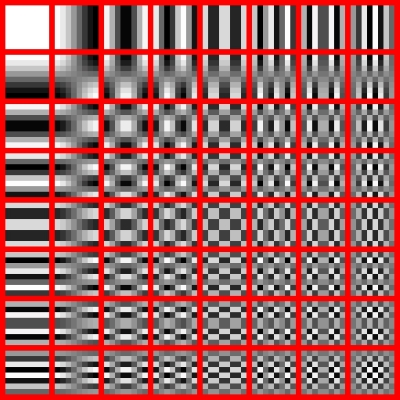
\includegraphics{DCT 2D.1} 
\end{center}
\paragraph{}\textit{These are the 64 cosine functions that can be combined to make any 8 by 8 image. }
\paragraph{}\textit{To generate an 8 by 8 image, it is necessary to incorporate a combination of all the cosine waves simultaneously. Each of these waves is assigned a coefficient, which denotes the magnitude of its contribution to the overall image. These coefficients serve as numerical representations of the relative importance of each individual cosine wave within the composition.  }
\paragraph{}\textit{So, what we do is basically is Centre all those values at 0, which were previously centered at 128. The reason for doing this is because the cosine wave ranges from –1 to 1, so we need negative values in our grey-scale. We subtract each value by 128, and get our shifted block.}
\paragraph{}\textit{We use these numbers to calculate our DCT coefficients. We use this formula given below to calculate our coefficients.}
\paragraph{}\\Formula for 1-D DCT coefficients:
\begin{center}
    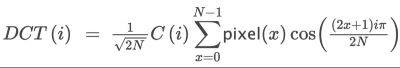
\includegraphics{F1} 
\end{center}
\paragraph{}Formula for 2-D DCT coefficients:
\begin{center}
    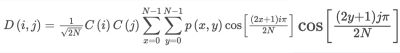
\includegraphics{F2.1} 
\end{center}
\paragraph{}C(u) = 1/\sqrt{2}\hspace{0.25cm} if\hspace{0.25cm}  u= 0,else\hspace{0.25cm} 1 \hspace{0.25cm} if\hspace{0.25cm}  u > 0.
\paragraph{}For JPEG we take N = 8.
\paragraph{}\textit{A notable advantage of the JPEG compression method is that the lower frequency cosine waves possess significantly larger coefficients compared to the higher frequency ones. DCT coefficients value ranges between –1024 to 1024.The top left coefficient is much bigger than others and so it is called direct current coefficient, or DC coefficient and all others are alternating current coefficients, or AC coefficients. }
\paragraph{}\textit{Important point to note that is the bottom right coefficients are very small and the top left coefficients are relatively larger. This observation indicates that the higher frequency cosine waves have minimal impact on the overall image representation. These frequencies have very subtle effect on actual output pixel data. These small weights are filtered out by quantization.}
\section{{\color{blue}Quantization}}
\paragraph{}\textit{Quantization is the compression of frequencies which are less visible to us (low contrast and high frequency). This is done by divide each of the DCT coefficients (frequency components) with some constants, followed by quantization. The frequency components which we are less sensitive to get divided by larger constants as compared to the ones we are more sensitive to. Quantization in this context simply means rounding off the results to the nearest integers.}
\paragraph{}\textit{Using larger divisors leads to more numbers rounding down to zero. This results in higher compression rates but also lowers the quality. }
\section{{\color{blue}Run-length encoding}}
\paragraph{}\textit{After quantization we end up with a lot of zeros in the high frequency. We rearrange the coefficients in a zig-zag order from top right to bottom left order to exploit redundancy, and store the information more efficiently. Once we get the zeros together, we can group them. Instead of storing each one of them separately we can store their value and number of times they occur consecutively occur in tuples.}
\begin{center}
    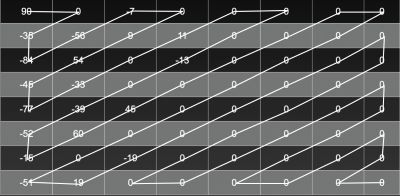
\includegraphics{Run1} 
\end{center}
\paragraph{}\textit{Further compression can be done by encoding the more frequent values with fewer bits and less frequent values with more bits. Doing this reduces the average number of bits per symbol. This process is called Huffman (entropy) coding.}
\paragraph{}\textit{Both run-length encoding and Huffman coding are lossless compression process, no information is lost in these processes. The compression is solely achieved by storing redundant data more efficiently. }
\section{{\color{blue}Huffman Coding}}
\paragraph{}\textit{Huffman coding is a vital component of the entropy coding stage in JPEG compression. Its purpose is to further compress the quantized DCT coefficients and other encoded data, resulting in a more efficient representation of the image.  }

\paragraph{}\textit{In the JPEG compression process, once the quantization step is completed, the resulting coefficients are arranged in a zigzag pattern to facilitate compression. While the run-length encoding (RLE) technique efficiently represents consecutive zeros, the resulting data still contains variable-length codes, which are not optimal for further compression.   }
\paragraph{}\textit{To address this, Huffman coding is employed to convert the variable-length codes into fixed-length codes known as Huffman codes. This encoding step significantly reduces the size of the compressed bitstream, making it more efficient for storage and transmission. }
\paragraph{}\textit{The Huffman coding in JPEG starts with a frequency analysis of the encoded data. Each unique symbol or code is examined, and its frequency of occurrence is determined. In the context of JPEG, these symbols represent the run lengths and categories of the quantized DCT coefficients. }
\paragraph{}\textit{Based on the frequency analysis, a Huffman tree is constructed in a bottom-up manner, beginning with individual symbols as leaf nodes. Symbols with the lowest frequencies are merged into parent nodes, creating a binary tree structure. This process continues until a single root node is formed. }
\paragraph{}\textit{Simultaneously with the tree construction, the encoding process takes place. Each symbol is assigned a binary code based on its position within the Huffman tree. Traversing the tree from the root to the leaf node corresponding to the symbol determines its binary code. Left branches represent the binary value "0," and right branches represent "1." The resulting binary codes assigned to each symbol form the Huffman codebook. }
\paragraph{}\textit{During compression, the original symbols are replaced with their respective Huffman codes. This substitution leads to a more compact representation of the data, with frequently occurring symbols represented by shorter codes and less frequent symbols represented by longer codes. The compressed bitstream consists of the sequence of Huffman codes for the encoded symbols. }
\paragraph{}\textit{During decompression, the reverse process takes place. The compressed bitstream is read bit by bit, and the Huffman codes are decoded by traversing the Huffman tree from the root to the appropriate leaf node. This decoding process converts the Huffman codes back into the original symbols, enabling the reconstruction of the encoded data. }
\paragraph{}\textit{Huffman coding is crucial for achieving efficient compression in JPEG. It converts variable-length codes into fixed-length Huffman codes, reducing the overall size of the compressed bitstream. By constructing a Huffman tree and assigning codes based on symbol frequencies, effective compression and decompression can be accomplished.}
\section{{\color{blue}Storage/Transmission}}
\paragraph{}\textit{After the JPEG image commpression , the compressed image data is obtained.This data consists of the quantized and encoded coefficients representing the image.The compressed image data is packed along with necessary meta data and parameters into a file format suitable for storage or transmission. The most common file format for JPEG compression is the JPEG File Interchange Format (.jpg).}
\paragraph{}\textit{The JPEG file format has a specific structure that consists of various sections and markers. These sections are used to organize the compressed image data and metadata. The file structure includes a header section, marker segments, and the compressed image data itself.}
\newpage
\section{{\color{blue}Decoding}}
\paragraph{}\textit{As the name suggests the decoding process is just the inverse of encoding process.Entropy decoding, much like entropy coding, can be conceptualized as a two-step procedure. Initially, the input bit stream is transformed into intermediate symbols during the first step. Subsequently, in the second step, these intermediate symbols are converted into quantized DCT coefficients. Specifically, the outcome of the second step encompasses the DC difference, which corresponds to the output of DPCM, as well as the AC coefficients following a zig-zag scan. Consequently, the DC difference is decoded to yield the quantized DC coefficient, while the AC coefficients are rearranged to restore their original order.}
\section{{\color{blue}Dequantization}}
\paragraph{}\textit{In the process of dequantization, what we do is basically multiply the DC  and AC coefficients with the same quantization table. We get a different  values as compared to the ones we get before quantization.The equation for Dequantization is :}
\begin{center}
    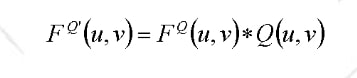
\includegraphics{Deq} 
\end{center}
\section{{\color{blue}Inverse Discrete Cosine Transform}}
\paragraph{}\textit{The last step of decoder is the IDCT. It takes the 64 quantized DCT coefficients and reconstructs a 64-point output image signal by summing the basis signals. JPEG does not specify a unique IDCT algorithm in its standard either.The equation of 8x8 IDCT is as followed:}
\begin{center}
    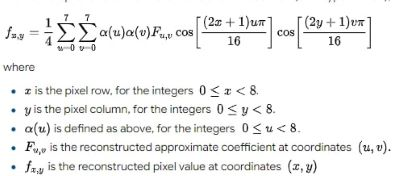
\includegraphics{IDCT.1} 
\end{center}
\paragraph{}\textit{After performing the inverse discrete cosine transform (IDCT), we add 128 to each block in the matrix to shift the values to the 0-255 range. Subsequently, the YCbCr values are converted back into the corresponding RGB values, and any necessary color space conversions or adjustments are applied. As a concluding step, the final image is obtained by merging the resulting RGB components with the chroma components.}
\section{{\color{blue}JPEG 2000}}
\paragraph{}\textit{It was published in the year 2000 and is the successor to the original JPEG standard, which was introduced in 1992. JPEG 2000 is designed to provide improved compression efficiency and higher image quality compared to its predecessor.}
\paragraph{}\textit{ Unlike the discrete cosine transform (DCT) used in JPEG, JPEG 2000 employs wavelet transformation for compression. This allows for better image quality preservation and the ability to store images at different levels of detail.}
\paragraph{}\textit{JPEG 2000 supports both lossy and lossless compression.Lossless compression ensurres the originality of the image while it's reconstruction from compressed data, while lossy compression sacrifices some data to achieve higher compression.}
\paragraph{}\textit{Despite it's advantages over JPEG 1992,JPEG 2000 has some disadvantages over it's previous version due to it's slower encoding and decoding time.}
\section{{\color{blue}Contribution}}
\begin{itemize}
  \item \textup{{\large Aditya Raina (202201466):} Documentation and Video.}
  \item \textup{{\large Om Lachake (202201017):} Documentation and Bibliography.}
  \item \textup{{\large Parjanya Rajput (202201115):} Presentation Slides and Matlab Code.}
  \item \textup{{\large Ayushi Jani (202201141):} Presentation Slides and Website.}
  \item \textup{{\large Pari Chauhan (202201189):} Website and Matlab Code.}
  \item \textup{{\large Harshali Dharmik (202201214):} Website and Video.}

\end{itemize}
\newpage
~\nocite{jaipur,pdf,Penn92,qoura,stanford-dct, reducible2022,baeldung2023,Bonix2018,Yuniblog}
\bibliographystyle{plain}
\bibliography{biblography.bib}
\end{document}